\chapter{レンダリングプロトコル}

3Dアプリケーションとコンポジッタとの間のプロトコルの中でも特に重要であるのが,
アプリケーションの表示に関するレンダリングプロトコルである.
レンダリングプロトコルに求められるものには以下のものがある.

\begin{itemize}
  \item 複数のアプリケーションが別々に提示してきたレンダリングの情報を合成して,
        1つの没入環境に矛盾なくレンダリングできる.
  \item 質の悪いアプリケーションが他のアプリケーションや環境全体に影響を及ぼさない.
        複数のアプリケーションを利用できる環境下では,質の悪いアプリケーションがあり,
        フレームレートにレンダリングが追いつかなかったり,ハングしてしまう可能性がある.
        このようなときにシステム全体への影響を最小限にする必要がある.
  \item レンダリングの効率がよい.
  \item レンダリングの自由度が高く,様々な表現が可能である.
        % \item Motion-to-photon(MTP) latency(ユーザが動いてから,その動きを反映させて
        %       レンダリングした結果の映像が目に届くまでの時間)を小さくできる.
        %       MTP latencyが大きくなるとVRやARにおけるPresenceの低下や
        %       motion sicknessを引き起こすと言われている.
        % 軽減手法を入れてもいいかも
\end{itemize}

\section{3Dコンピュータグラフィックス}
\label{section:3DCG}

この節では以降の説明のために最小限必要な,3Dレンダリングにおけるレンダリングパイプラインの
概要を述べる.
ただしレンダリングの手法は様々であり,ここでは代表的な手法についてのみ述べている.

3Dオブジェクトのレンダリングは基本的に,3D空間で定義されたオブジェクトを,ある視点から見た
時の2次元平面でのピクセルマップに落とし込む行為である.
このプロセスは大きく,Geometry ProcessingとRasterizationの2つのフェーズに
分けることができる.

\subsection*{Geometry Processing}

3Dオブジェクトの形は多くの場合,メッシュによって表現され.メッシュは三角形などのPrimitiveの
集まりとして表現される.
レンダリングパイプラインではこのPrimitiveごとに,それがScreenのどのピクセルを何色で
塗りつぶすかを計算する.
Geometry Processingのフェーズ(図\ref{fig:geometry-processing})
ではこのPrimitiveを構成する頂点の座標(Object Space)を行列計算によって,
ある視点から投影したときの座標(Clip Space)へ変換するフェーズである.
Primitiveの頂点はまず,Model Matrixをかけることで,World Spaceのどこに配置するかが決定される.
さらにこれに,視点の位置や向き,視野角などから取得されるView Projection Matrixを乗算することで,
頂点はClip Spaceに配置される.

これらの操作はVertex Shaderによって制御される.OpenGL
\footnote{Khronos Group "OpenGL" https://www.opengl.org/ (accessed 27 Dec, 2022)}
のシェーダ言語であるGLSLにおける簡単なVertex Shaderの例を
ソースコード\ref{code:vertex-shader}に示した.
ここでのmodel,view\_projectionの値はレンダリングパイプラインを実行するときに
プログラマが指定できる.

\begin{figure}[htbp]
  \centering
  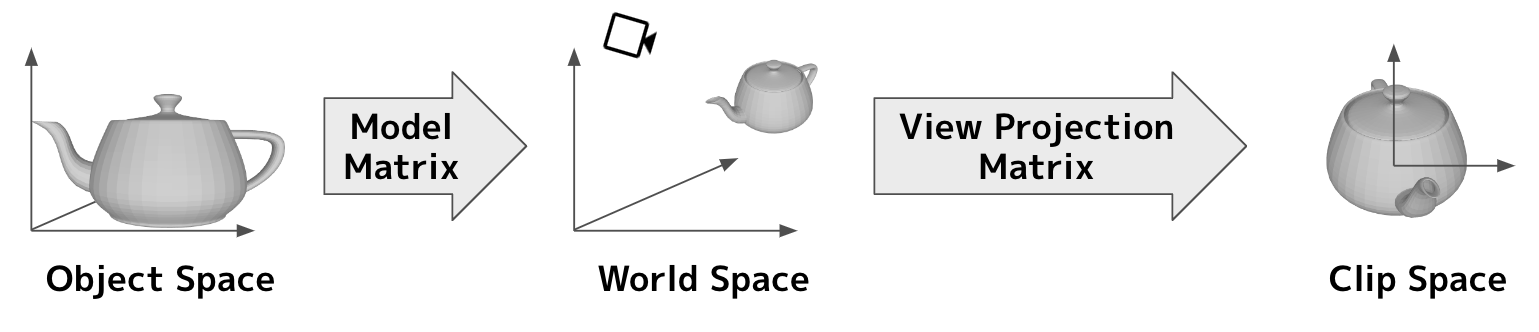
\includegraphics[keepaspectratio, width=\linewidth]{figures/geometry-processing.png}
  \caption{
    Geometry Processing.
  }
  \label{fig:geometry-processing}
\end{figure}

\begin{lstlisting}[caption=Vertex Shaderの例, label=code:vertex-shader]
uniform mat4 model;
uniform mat4 view_projection;
layout(location = 0) in vec4 position;

void main() {
  gl_Position = view_projection * model * position;
}
\end{lstlisting}

\subsection*{Rasterization}

Clip Spaceに変換されたPrimitiveはRasterizationのプロセスによって,
スクリーン上のどのピクセルをどの色で塗るかといった情報にまで落とし込む.
このピクセルごとの情報はフラグメントと呼ばれ,一般的にフラグメントには色の情報と,
そのフラグメントに投影されたPrimitiveが視点からどれくらい離れているかを指す深度情報が含まれる.
このRasterizationのフェーズではFragment Shaderやテクスチャなどをプログラマが指定する.

\subsection*{Framebuffer と Depth Testing}

Framebufferとはレンダリング結果を格納するバッファである.
Framebufferはピクセルごとの色の情報を保持するColor bufferと
深度の情報を保持するDepth bufferを含むことが多く,Rasterizationによって得られた
フラグメントはFramebufferのColor bufferとDepth bufferに格納される.
RasterizationによってPrimitiveがフラグメントに変換され,そのフラグメントが次々と
Framebufferに書きこまれていくが,このときDepth Testingを用いると,
フラグメントの深度情報とFramebufferが持つ深度情報とを比較して,
フラグメントが手前にあるときだけ,Framebufferに書き込むということができる.
これによって,重なっているPrimitiveの処理順に関係なく,Primitiveの前後関係を
レンダリングに反映させている.

\subsection*{レンダリングパイプライン}

今まで述べたプロセスはレンダリンパイプラインとして,GPU内で行われることが多い.
ただしレンダリングパイプラインを実行するために必要なデータはプログラマによって
CPUで作成され,OpenGLなどのAPIを通してGPUに送られるのが一般的である.
レンダリングパイプラインへの入力としては主に以下のものがある.

\begin{itemize}
  \item メッシュに関するデータ:頂点の位置情報やそれに付随するデータなど.
  \item テクスチャ
  \item Model Matrix の値
  \item View Projection Matrix の値
  \item Vertex / Fragment Shader
\end{itemize}

\section{関連技術・研究}

本システムはそれぞれ別プロセスのアプリケーションがレンダリングしたい情報を持っており,結果的に
1つのレンダリング結果を導くという点でParallel Renderingの分野と類似性がある.
MolnarらはParallel Renderingの手法を``sort-first'', ``sort-middle'', ``sort-last''の
大きく3つに大別した\cite{parallel-rendering}(図\ref{fig:parallel-rendering}).
\ref{section:3DCG}で述べたとおり,3DレンダリングはPrimitiveがどのピクセルに影響を与えるかを
計算するタスクであり,Primitiveをスクリーンへとsort(選別・分配)するタスクであると捉えられる.
Parallel Renderingにおいてこのsortのタスクでは,プロセッサ間でPrimitiveやフラグメントに
関するデータを再配置する必要がある.
Molnarらはこの再配置のタイミングに注目しており,``sort-first''は,Primitiveを
Geometry Processingの際に再配置する手法,``sort-middle''はGeometry Processing後の
Primitiveを再配置する手法,そして``sort-last''はRasterizationの際にフラグメントなどを
再配置する手法である.

\begin{figure}[htbp]
  \begin{minipage}[t]{0.32\linewidth}
    \centering
    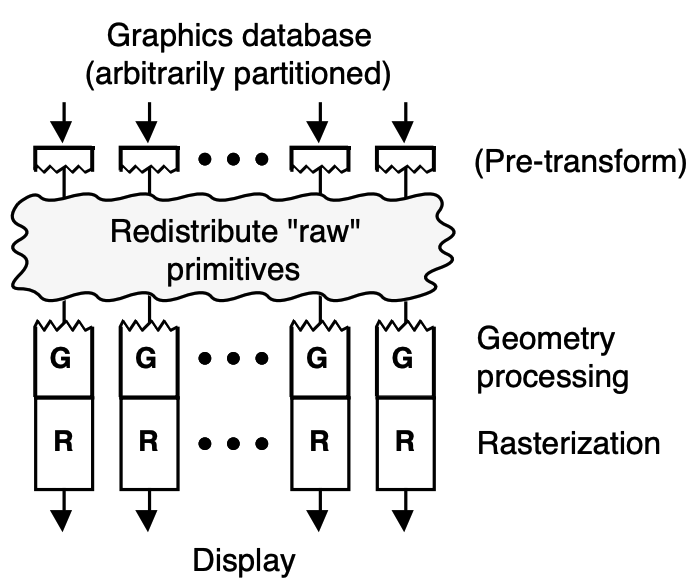
\includegraphics[keepaspectratio, width=\linewidth]{figures/sort-first.png}
    \subcaption*{Sort-first}
  \end{minipage}
  \begin{minipage}[t]{0.32\linewidth}
    \centering
    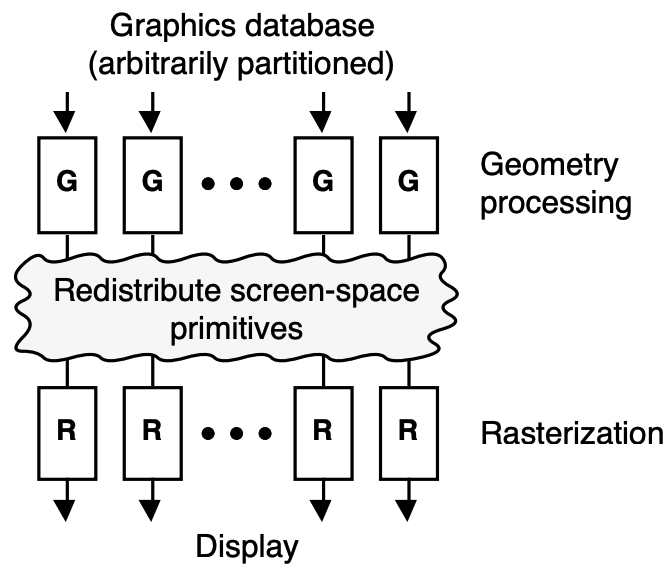
\includegraphics[keepaspectratio, width=\linewidth]{figures/sort-middle.png}
    \subcaption*{Sort-middle}
  \end{minipage}
  \begin{minipage}[t]{0.32\linewidth}
    \centering
    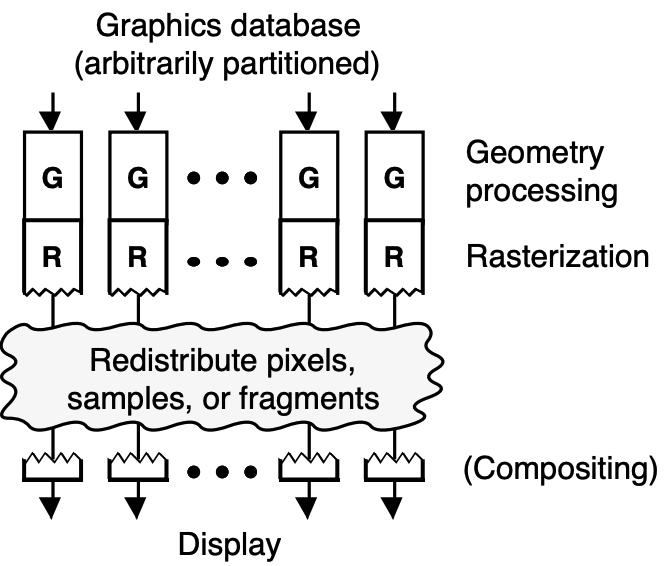
\includegraphics[keepaspectratio, width=\linewidth]{figures/sort-last.png}
    \subcaption*{Sort-last}
  \end{minipage}
  \caption{
    Molnarらによって分類されたParallel Renderingの3つの手法.
    (Each figure is adapted from Molnar, at el. 1994\cite{parallel-rendering})
  }
  \label{fig:parallel-rendering}
\end{figure}

本研究では,複数のアプリケーションがコンポジッタに対してレンダリングに必要な情報を伝達して,
それを用いてコンポジッタ側が最終的なレンダリングを行うため,Molnarらの分類において,
データの分配のタイミングまでをアプリケーションが担い,分配後をコンポジッタが担うと捉えられる.
ただしMolnarらの設定とは大きな違いがあり,Molnarらの論文ではスクリーンはいくつかの領域に
分割され,その領域ごとにプロセッサが割り当てられてレンダリングを行う設定であったため,
どのプロセッサにデータを再配置するかを知るために,データがスクリーンのどの領域に
影響を与えるものであるか計算できている必要があった.
一方本研究の設定では,アプリケーションがデータを作成しコンポジッタで合成するために
データの再配置(アプリケーションからコンポジッタへの描画情報の伝達)をおこなう.
全く異なる設定ではあるが,Molnarらの論文での洞察や検証は本研究にも応用できる部分が多い.

Reilingの提案したmotorcar\cite{reiling}は
``sort-last''に近い手法(図\ref{fig:reiling-rendering})をとっている.
motorcarではそれぞれのアプリケーション(図\ref{fig:reiling-rendering}ではclient)が
レンダリングを行い,生成したフレームバッファをできるだけ効率のよい方法でコンポジッタに送り,
Depth Testingによってそれぞれのアプリケーションのフレームバッファどうしを合成している.
motorcarの手法の特徴は以下のとおりである.

\subsubsection*{矛盾のないレンダリングについて}

Depth Testingによって,複数のアプリケーションを矛盾なく合成できる.

\subsubsection*{質の悪いアプリケーションについて}

質の悪いアプリケーションがフリーズしてしまった場合などは,オブジェクトが消えてしまうか,
視点の情報を更新できず,描画の整合性が失われてしまう.

\subsubsection*{レンダリングの効率について}

複数のアプリケーションがGPUを共有するため,プロセス間でGPUを奪い合い,
コンテキストスイッチにオーバヘッドがある.
また,Molnarらが指摘しているとおり,``sort-last''の手法ではコンポジッタに対して毎フレーム
全てのフラグメントの情報を送る必要があり,データの転送量が多くなってしまう.
Reilingの手法では単一ホストマシン内でのデータ転送であるため,アプリケーションとコンポジッタで
共有したバッファを用いることで時間がかかるGPUメモリへの読み書きを最小限に抑え,
伝達効率を上げているが,Reiling自身が言及されているとおり,
バッファへの書き込みや読み出しの部分でオーバヘッドが存在する.

\subsubsection*{レンダリングの自由度について}

アプリケーションがレンダリングパイプラインを全て実行できるため,描画の自由度が高い.
ただし,他のアプリケーションのオブジェクトの形などの情報は取得できないため,
他のアプリケーションの影を落とすといったことはできない.

% \subsubsection*{MTP latencyについて}

% motorcarではHMDなどのデバイスから取得される視点の情報がアプリケーションに伝えられ,
% アプリケーションでレンダリングを行って結果がコンポジッタに戻ってくる.
% このため,コンポジッタ側では最低でも次のフレームタイミングよりも,
% アプリケーションで行われるレンダリングの時間分だけ早くその視点の情報を伝える必要がある.
% しかしこの時間を短く見積もってしまうと,アプリケーションのレンダリングが間に合わず,
% フレーム落ちを発生させてしまう.

\begin{figure}[htbp]
  \centering
  \fbox{
    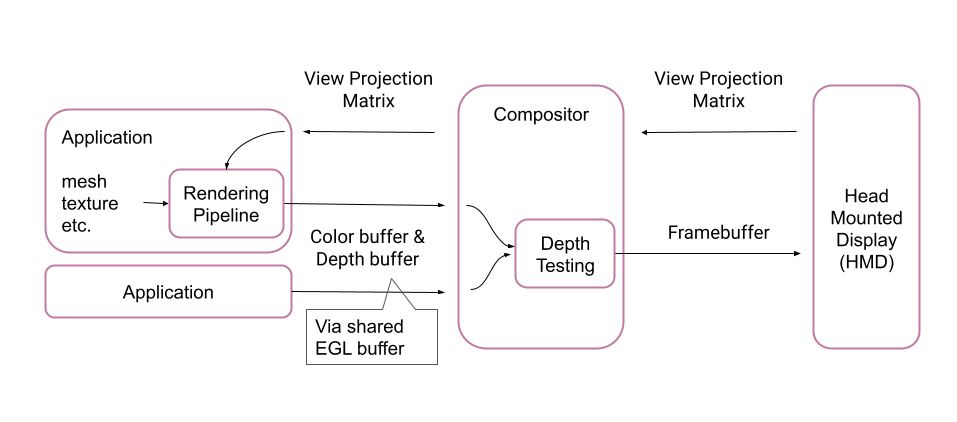
\includegraphics[keepaspectratio, width=0.9\linewidth]{figures/reiling-rendering.png}
  }
  \caption{
    motorcar\cite{reiling}でのレンダリング手法の概略図.
  }
  \label{fig:reiling-rendering}
\end{figure}

Peuhkurinenらはmotorcarの手法におけるコンテキストスイッチのオーバヘッドを指摘し,
アプリケーションとコンポジッタとの間で共有したシーングラフを用いる手法を提案した\cite{peuhkurinen}.
Peuhkurinenらはモバイル端末を用いたAR環境で実験をしているため,没入環境ではないが,
端末の位置や傾きをもとに,複数のアプリケーションをAR環境にレンダリングしている点で,
レンダリングに関しては本研究と同じ問題に取り組んでいる.
Peuhkurinenらの手法(図\ref{fig:peuhkurinen-rendering})ではコンポジッタ側で
1つのシーングラフを持ち,アプリケーションがIPCによってそのシーングラフに変更を加える.
コンポジッタでは毎フレームそのシーングラフを走査し,そのタイミングで取得した
デバイスの位置や傾きを使ってシーンをレンダリングする.
Peuhkurinenらの手法の特徴は以下のとおりである.

\subsubsection*{矛盾のないレンダリングについて}

システムで共有するシーングラフからレンダリングすることで
複数のアプリケーションを矛盾なくレンダリングできる.

\subsubsection*{質の悪いアプリケーションについて}

質の悪いアプリケーションがフリーズした場合でも,シーングラフの更新が途絶えるだけで,
フレームごとにデバイスの位置や傾きを更新して,矛盾なくシーンをレンダリングできる.

\subsubsection*{レンダリングの効率について}

レンダリングは全てコンポジッタ側で行われるため,
コンテキストスイッチのオーバヘッドがなく効率的である.

\subsubsection*{レンダリングの自由度について}

シーングラフの設計によってレンダリングできるものが限られてしまい,レンダリングの自由度は
著しく落ちる.
特にPeuhkurinenらが提案したシーングラフを構成する要素は以下の5つであり,
より高度なレンダリングを実現する提案までは至らなかった.

\begin{enumerate}
  \item \textbf{Mesh}
        位置を表す(X,Y,Z)と頂点の法線ベクトルの(X,Y,Z),UVマッピングのための(U,V)の情報を持つ.
  \item \textbf{Texture}
        8bitずつのRGBAのコンポーネントを持つ.
  \item \textbf{Transformation Matrix}
        アプリケーションのローカル座標系におけるMeshの平行移動,回転,スケールを表す4x4の変換行列.
  \item \textbf{Node}
        Mesh,Texture,Transformation Matrixから構成され,コンポジッタによって描画される単位.
  \item \textbf{Application Volume}
        アプリケーションがNodeを描画できる直方体領域.
\end{enumerate}

\begin{figure}[htbp]
  \centering
  \fbox{
    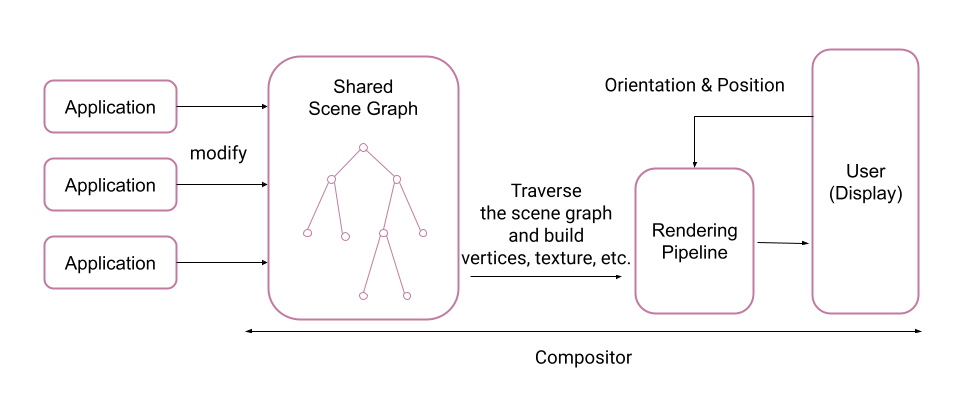
\includegraphics[keepaspectratio, width=0.9\linewidth]{figures/peuhkurinen-rendering.png}
  }
  \caption{.
    Peuhkurinenら\cite{peuhkurinen}の提案するシステムのレンダリング手法の概略図.
  }
  \label{fig:peuhkurinen-rendering}
\end{figure}

% sort-first か sort-last かみたいな有名な論文から
% http://www.cs.cmu.edu/afs/cs/academic/class/15869-f11/www/readings/molnar94_sorting.pdf?fbclid=IwAR1oupZA71Gn8IAoOu0F5fJ-GbjJjJH6moYND0nTmtw0w81hqK1qpen7TR4
% Forrestなど、似たことをしようとしているものも

\section{提案手法}

% 視点情報を送らない

\section{評価}

% 実験内容
% * レンダリング性能
% * 自由度
% Limitation

\section{結論}

% * 今後の展開
% ** PBR ベースなど
